% =============================================================================
% CardSiege -- Schriftliche Ausarbeitung
% Modul: Design Pattern in der OOP
% Kompiliere mit: lualatex Doku.tex
% =============================================================================
\documentclass[a4paper,12pt]{article}

\usepackage[ngerman]{babel}
\usepackage[left=2.5cm, right=2.5cm, top=2.5cm, bottom=2.5cm]{geometry}
\usepackage{parskip}
\usepackage{fancyhdr}
\setlength{\headheight}{14.5pt}
\usepackage{graphicx}
\usepackage{float}
\usepackage{booktabs}
\usepackage{array}

\usepackage[
    colorlinks=true, linkcolor=black, urlcolor=blue, citecolor=black,
    pdftitle={CardSiege -- Design Pattern in der OOP},
    pdfauthor={Sven Sinowcz6ik}
]{hyperref}

\usepackage{amsmath}
\usepackage{xcolor}
\usepackage{listings}

\definecolor{codegray}{rgb}{0.5,0.5,0.5}
\definecolor{codegreen}{rgb}{0,0.5,0}
\definecolor{backcolour}{rgb}{0.95,0.95,0.95}

\lstset{
    language=Java,
    backgroundcolor=\color{backcolour},
    basicstyle=\ttfamily\small,
    keywordstyle=\color{blue}\bfseries,
    stringstyle=\color{codegreen},
    commentstyle=\color{codegray}\itshape,
    numberstyle=\tiny\color{codegray},
    numbers=left, numbersep=8pt,
    breaklines=true, showstringspaces=false,
    frame=single, framerule=0.5pt, rulecolor=\color{codegray},
    tabsize=4, captionpos=b,
    xleftmargin=1.5em, framexleftmargin=1.5em,
    aboveskip=0.8em, belowskip=0.8em,
    keepspaces=true, columns=fixed,
    literate={ä}{{\"a}}1 {ö}{{\"o}}1 {ü}{{\"u}}1
             {Ä}{{\"A}}1 {Ö}{{\"O}}1 {Ü}{{\"U}}1 {ß}{{\ss}}1
}

\pagestyle{fancy}
\fancyhf{}
\fancyhead[L]{\small CardSiege -- Design Pattern in der OOP}
\fancyhead[R]{\small \textit{[Kurskennung]}}
\fancyfoot[C]{\thepage}
\renewcommand{\headrulewidth}{0.4pt}

\usepackage{microtype}
\clubpenalty=10000
\widowpenalty=10000

% =============================================================================
\begin{document}
\pagenumbering{Alph}

\begin{titlepage}
    \centering
    \vspace*{2cm}
    {\Huge\bfseries CardSiege\par}
    \vspace{0.5cm}
    {\Large Rundenbasiertes Kartenspiel mit Tower-Defense-Mechaniken\par}
    \vspace{0.3cm}
    {\large Implementierung von neun GoF-Design-Patterns in Java/libGDX\par}
    \vspace{2cm}
    {\large Schriftliche Ausarbeitung\par}
    \vspace{0.3cm}
    {\large im Modul \textbf{Design Pattern in der OOP}\par}
    \vspace{2cm}
    \begin{tabular}{rl}
        \textbf{Autor:}    & Sven Sinowczik (Matr.-Nr. 30422906) \\

        \textbf{Hochschule:} & FH Südwestfalen \\[0.5em]
        \textbf{Datum:}      & \today \\
    \end{tabular}
    \vfill
\end{titlepage}

\clearpage
\pagenumbering{arabic}
\tableofcontents
\newpage

% =============================================================================
% Kapitel 1 -- Einleitung
% =============================================================================
\section{Einleitung}

\subsection{Motivation}

Entwurfsmuster sind bewährte Lösungsschablonen für wiederkehrende Probleme in der
objektorientierten Softwareentwicklung. Das Standardwerk der \textit{Gang of Four}
(Gamma et al., 1994) hat sie als gemeinsame Sprache für Architekturentscheidungen
etabliert. Ihr eigentlicher Wert zeigt sich jedoch erst im Kontext eines realen
Entwurfsproblems, die reine Theorie lässt ihren Nutzen oft abstrakt wirken.

Dieses Projekt setzt neun GoF-Patterns in \textbf{CardSiege} um, einem
rundenbasierten Kartenspiel mit Tower-Defense-Mechaniken in Java und libGDX.
Spieleentwicklung ist ein besonders geeignetes Anwendungsgebiet: Spiele verwalten
komplexe, sich ständig ändernde Zustände, viele Objekte interagieren eng
miteinander, und Erweiterbarkeit ist von Anfang an gefordert. Jedes eingesetzte
Pattern löst dabei ein konkretes Architekturproblem, das sich ohne das Muster in
Kopplung, Codeduplikation oder mangelnder Wartbarkeit niedergeschlagen hätte.

\subsection{Spielkonzept}

Der Spieler verteidigt eine Basis gegen zwölf Gegnerwellen, indem er auf einem
20$\times$20-Rasterfeld strategisch Türme platziert. Das Besondere liegt im
kartenbasierten Ressourcensystem: Statt Türme direkt zu kaufen, zieht der Spieler
zu Beginn jeder Runde drei Karten aus einem gemischten Deck. Diese ermöglichen
unterschiedliche Aktionen, Turmbau, Attribut-Buffs, Ressourcengewinn oder
Sondereffekte wie das Verlangsamen von Gegnern.

Jeder Spielzug folgt einem festen Viererzyklus: \textit{Draw} (Karten ziehen,
Energie auffüllen) $\rightarrow$ \textit{Play} (Karten ausspielen, Türme
positionieren) $\rightarrow$ \textit{Wave} (Gegnerwelle läuft, Türme greifen
automatisch an) $\rightarrow$ \textit{Resolve} (kurze Pause, nächster Zug
beginnt). Das Spiel endet mit Sieg nach zwölf abgewehrten Wellen oder mit
Niederlage, sobald die Basis auf null Lebenspunkte fällt. 
\newpage
% =============================================================================
% Kapitel 2 -- Anforderungen und Pattern-Auswahl
% =============================================================================
\section{Anforderungen und Pattern-Auswahl}

Das Spiel erfüllt alle funktionalen Anforderungen: drei Turmtypen (Scout, Sniper,
Rapid), drei Gegnertypen (Standard, Fast, Tank) mit unterschiedlichen
Geschwindigkeiten und Trefferpunkten, ein vollständiger Rundenzyklus mit vier
Phasen sowie zehn verschiedene Kartentypen für Bau, Buffs und Sonderaktionen.
Grafisch dargestellt wird das Spiel über libGDX mit Spielfeld, HUD und
Kartenhand. Nicht-funktional wurde auf Modularität und Erweiterbarkeit geachtet:
Abhängigkeiten verlaufen über Interfaces, neue Karten- oder Turmtypen lassen sich
ohne Änderung bestehenden Codes ergänzen. Das Spielsystem
wurde in Java~21 mit libGDX umgesetzt und per Gradle gebaut;
Lombok reduziert Boilerplate durch \texttt{@Getter}-Annotationen.

Die Auswahl der neun GoF-Patterns folgt direkt aus den Anforderungen -- jedes
Muster löst ein identifizierbares Entwurfsproblem. Tabelle~\ref{tab:patterns}
gibt einen Überblick.

\begin{table}[H]
\centering
\begin{tabular}{llp{7.5cm}}
\toprule
\textbf{Pattern} & \textbf{Kategorie} & \textbf{Gelöstes Problem} \\
\midrule
Singleton      & Erzeugung & Exakt eine konsistente Spielzustandsinstanz \\
Factory Method & Erzeugung & Deck kennt keine konkreten Kartentypen \\
Prototype      & Erzeugung & Konfigurierte Objekte klonen statt neu aufbauen \\
Builder        & Erzeugung & Turmkonfiguration vor Platzierung trennen \\
Decorator      & Struktur  & Türme zur Laufzeit stapelbar erweitern \\
Command        & Verhalten & Kartenaktionen als eigenständige Objekte kapseln \\
Strategy       & Verhalten & Zielwahl und Angriffstyp unabhängig kombinieren \\
State          & Verhalten & Phasenverhalten ohne if-else-Ketten verwalten \\
Observer       & Verhalten & Ereignisse entkoppelt von reaktiven Systemen \\
\bottomrule
\end{tabular}
\caption{Übersicht der neun implementierten GoF-Design-Patterns}
\label{tab:patterns}
\end{table}


Besonders hervorzuheben ist die Aufteilung in vier Erzeugungsmuster, die gemeinsam
die gesamte Objekterzeugung des Spiels abdecken, und vier Verhaltensmuster, die
das laufende Spielgeschehen strukturieren. Das Decorator-Pattern als einziges
Strukturmuster nimmt dabei eine Sonderrolle ein: Es ist das architektonisch
prägendste Muster des Projekts und kooperiert eng mit Command und Strategy.

\newpage
% =============================================================================
% Kapitel 3 -- Architektur & Design Patterns
% =============================================================================
\section{Architektur}

\subsection{Der GameManager als zentraler Koordinator}

Der \texttt{GameManager} ist das Herzstück von CardSiege. Er hält Referenzen auf
alle wesentlichen Spielobjekte: Spielfeld, Türme, Gegner, Projektile,
Kartensystem, aktuelle Phase, Ressourcen und den Ereignisbus und orchestriert
deren Zusammenspiel. Seine zentrale \texttt{update()}-Methode wird einmal pro
Frame vom \texttt{GameScreen} aufgerufen und koordiniert Gegnerbewegung,
Reichweitenüberwachung, Kampflogik und das Aufräumen besiegter Einheiten.
Sämtliche inhaltliche Verantwortung delegiert er dabei an spezialisierte
Teilsysteme, deren konkrete Umsetzung er nicht kennt. Wie diese Delegation
architektonisch strukturiert ist, beschreiben die folgenden Abschnitte.

% =============================================================================
\subsection{Singleton - GameManager}
% =============================================================================

Ein Tower-Defense-Spiel besitzt zu jedem Zeitpunkt genau einen definierten
Spielzustand. Turmlisten, Phasenzustand, Ressourcenzähler und der aktive
Ereignisbus müssen konsistent von einer einzigen Stelle verwaltet werden.
Würden mehrere \texttt{GameManager}-Instanzen existieren, könnten Türme in einer
Instanz registriert, Gegner aber in einer anderen verwaltet werden, das Spiel
wäre nicht mehr deterministisch steuerbar.

Der \texttt{GameManager} wird deshalb als Singleton mit \textit{Eager
Initialization} umgesetzt: Die einzige Instanz entsteht als statische
Klassenvariable beim Klassenladen der JVM, noch bevor irgendein Aufruf von
\texttt{get()} möglich ist. Ein privater Konstruktor verhindert externe
Instanziierung vollständig. Diese Variante wurde der lazy Alternative
(\texttt{if (INSTANCE == null)}) vorgezogen, weil das Spiel single-threaded
läuft und eine aufwändige Synchronisierung unnötig wäre.

\begin{lstlisting}[caption={Singleton mit Eager Initialization},label=lst:singleton]
public class GameManager {
    private static final GameManager INSTANCE = new GameManager();

    public static GameManager get() { return INSTANCE; }

    private GameManager() {
        eventBus.subscribe(new GameEventLogger()); // Observer sofort aktiv
    }
}
\end{lstlisting}

Bemerkenswert ist, dass der Konstruktor unmittelbar das Observer-System
initialisiert: Der \texttt{GameEventLogger} wird bereits im privaten Konstruktor
am \texttt{GameEventBus} registriert, sodass das Logging-System von der ersten
Spielaktion an aktiv ist, ohne explizite Initialisierungsreihenfolge nach außen.
Der bekannte Nachteil erschwerter Unit-Tests durch persistierenden globalen Zustand
wurde zugunsten der Einfachheit akzeptiert. In einem produktiven Kontext würde man
den \texttt{GameManager} per Dependency Injection übergeben.

% =============================================================================
\subsection{Factory Method - CardFactory}
% =============================================================================

Das Deck soll Karten erzeugen, ohne konkrete Kartentypen zu kennen. Wäre die
Erzeugungslogik direkt in der \texttt{Deck}-Klasse implementiert, würde jede
neue Karte eine Änderung im Deck-Code erzwingen, eine direkte Verletzung des
Open/Closed Principle. Das Problem liegt darin, dass Erzeugung und Verwaltung
von Karten zwei grundlegend verschiedene Verantwortlichkeiten sind, die
voneinander getrennt gehören.

Das Interface \texttt{CardFactory} definiert eine einzige Methode
\texttt{createDeck()}, die eine Liste fertig konfigurierter Karten zurückgibt.
Das \texttt{Deck} kennt ausschließlich dieses Interface, nie eine konkrete
Kartenklasse. Die gesamte Entscheidung darüber, welche Karten mit welchen
Parametern im Deck landen, liegt in der konkreten Implementierung
\texttt{StrategyCardFactory}. Diese bestückt das Deck mit zehn Kartentypen: drei
Turmkarten (Scout, Sniper, Rapid) mit ihren jeweiligen Strategie-Kombinationen
sowie sieben Karten für Ressourcen, Buffs und Sondereffekte. Ein alternativer
Kartensatz für einen anderen Schwierigkeitsgrad oder ein Tutorial ließe sich
vollständig durch eine neue \texttt{CardFactory}-Implementierung einführen, ohne
eine einzige Zeile in \texttt{Deck} zu ändern.

\begin{lstlisting}[caption={Factory-Interface und Nutzung im Deck},label=lst:factory]
public interface CardFactory {
    List<Card> createDeck();
}

// Deck kennt nur das Interface, nie konkrete Kartenklassen:
private void refill() {
    for (Card proto : factory.createDeck()) {
        cards.add(proto.copy()); // Prototype Pattern
        cards.add(proto.copy());
    }
    Collections.shuffle(cards);
}
\end{lstlisting}

Das unmittelbare Zusammenspiel mit dem Prototype-Pattern ist an dieser Stelle
besonders deutlich: Die Factory liefert konfigurierte Prototypen, das Deck klont
jeden zweimal, um zwanzig Karten zu erhalten. Weder Deck noch Factory wissen
voneinander, wie die Objekte intern konstruiert sind.

% =============================================================================
\subsection{Prototype - Card.copy() und EnemyPrototype}
% =============================================================================

Das Prototype-Pattern adressiert in CardSiege dasselbe konzeptionelle Problem an
zwei verschiedenen Stellen: Konfigurierte Objekte sollen geklont werden, anstatt
ihre Parameter bei jeder Erzeugung erneut angeben zu müssen. Ohne Prototype
müsste die Konfiguration, etwa Geschwindigkeit und Trefferpunkte eines
Gegnertyps, an jeder Spawn-Stelle im Code wiederholt werden, was zu
Inkonsistenzen führen und Änderungen aufwändig machen würde.

Im Kartensystem schreibt die abstrakte Basisklasse \texttt{Card} die Methode
\texttt{copy()} vor, die jede konkrete Kartenklasse implementiert. Das Deck ruft
\texttt{copy()} beim Befüllen auf und erhält so frische Instanzen mit identischem
Zustand, die aber voneinander unabhängig sind, das Ausspielen einer Karte
beeinflusst keinen anderen Kartenstapel. Die Klon-Logik im Deck bleibt dabei
stabil, egal wie viele neue Kartentypen hinzukommen.

Im Gegnersystem hält der \texttt{WaveSpawner} drei konfigurierte
\texttt{EnemyPrototype}-Objekte, einen für jeden Gegnertyp. Die Attribute werden
einmal pro Welle festgelegt und skalieren mit der Wellennummer. Bei jedem
Spawn-Vorgang wird der passende Prototyp über \texttt{copy(path)} geklont,
wobei der aktuelle Spielfeldpfad mitgegeben wird, da jeder Gegner seinen eigenen,
unabhängigen Fortschritt auf dem Pfad verfolgt.

\begin{lstlisting}[caption={Prototype im WaveSpawner},label=lst:prototype]
// Einmalig pro Welle konfiguriert:
standardEnemy = new EnemyPrototype(EnemyType.STANDARD, baseSpeed, baseHp);

// Pro Spawn geklont, Konfiguration zentral, Pfadfortschritt immer frisch:
manager.spawnEnemy(selectPrototype(index).copy(manager.getBoard().getPath()));
\end{lstlisting}

Dass dasselbe Pattern an zwei unabhängigen Stellen eingesetzt wird, illustriert
seine Vielseitigkeit. In beiden Fällen liegt der Kern des Problems nicht in der
Erzeugung an sich, sondern in der zentralen Verwaltung von Konfiguration: Es
soll eine einzige, verlässliche Quelle der Wahrheit für die Eigenschaften eines
Objekttyps geben.

% =============================================================================
\subsection{Builder - PendingTower}
% =============================================================================

Wenn der Spieler eine Turmkarte ausspielt, ist zu diesem Zeitpunkt ein
wesentlicher Parameter noch unbekannt: die Gitterkoordinaten, auf denen der
Turm platziert werden soll. Der Spieler muss erst auf ein gültiges Spielfeld-Feld
klicken. Eine direkte Erzeugung des Turms beim Kartenspielen ist damit nicht
möglich, der Bauprozess ist zwingend zweistufig.

Das Builder-Pattern trennt deshalb die Konfiguration des Turms von seiner
Instanziierung. Wenn eine \texttt{BuildTowerCard} ausgespielt wird, erzeugt sie
einen \texttt{PendingTower}, der alle bereits bekannten Parameter speichert:
Name, Typ, Kosten, Basisschaden, Reichweite, Cooldown sowie die gewählten
Targeting- und Angriffsstrategien. Ein \texttt{BaseTower} wird zu diesem
Zeitpunkt noch nicht erzeugt. Erst wenn der Spieler auf ein gültiges Feld
klickt, ruft der Manager \texttt{PendingTower.build(gridX, gridY)} auf und
übergibt die nun bekannten Koordinaten.

\begin{lstlisting}[caption={Zweistufige Turmerzeugung mit PendingTower},label=lst:builder]
// Schritt 1 - Karte ausgespielt, Koordinaten noch unbekannt:
context.getManager().queueTowerPlacement(new PendingTower(...));

// Schritt 2 - Spieler klickt Zielfeld, Koordinaten jetzt bekannt:
public TowerComponent build(int gridX, int gridY) {
    return new BaseTower(name, type, gridX, gridY, baseDamage,
                         range, cooldown, cost, targeting, attackStrategy);
}
\end{lstlisting}

Diese Trennung hat einen praktischen Nebennutzen, der direkt aus der
Architekturentscheidung erwächst: Solange ein \texttt{PendingTower} aktiv ist,
rendert der \texttt{GameScreen} einen Platzierungsmarker mit Reichweitenkreis
auf dem Spielfeld. Der Spieler sieht visuell, welchen Bereich der Turm abdecken
würde, bevor er die endgültige Entscheidung trifft, ohne dass dafür ein echter
Turm existieren müsste. Das Builder-Pattern liefert hier also nicht nur
sauberere Objekterzeugung, sondern ermöglicht direkt ein UI-Feature.

% =============================================================================
\subsection{Decorator - Turmerweiterungssystem}
% =============================================================================

Das Decorator-Pattern ist die architektonisch prägendste Entscheidung im Projekt,
weil sie ihren Nutzen im direkten Vergleich zur Alternative am deutlichsten
demonstriert. Türme sollen zur Laufzeit mit Boni ausgestattet werden können:
Eine Buff-Karte erhöht den Schaden aller Türme, eine andere erhöht die Reichweite
eines einzelnen Turms, ein Upgrade verbessert Level, Schaden und Cooldown
gleichzeitig. Diese Boni können in beliebiger Reihenfolge und Kombination
auf einen Turm angewendet werden.

Die naheliegende Alternative wäre Vererbung: Für jede mögliche Kombination aus
Turmtyp und Buffzustand eine eigene Klasse. Mit drei Turmtypen und drei Bufftypen
wären das bereits 24 Klassen, die bei jedem neuen Bufftyp weiter explodieren.
Das Decorator-Pattern löst dieses Problem fundamental anders: Alle Türme und alle
Dekoratoren implementieren dasselbe Interface \texttt{TowerComponent}. Die
abstrakte Klasse \texttt{TowerDecorator} hält eine Referenz auf ein inneres
\texttt{TowerComponent} und delegiert alle Methoden per Default daran. Konkrete
Dekoratoren überschreiben ausschließlich die Methoden, für die sie einen Bonus
liefern.

\begin{lstlisting}[caption={Delegation und gezielte Überschreibung im Decorator},label=lst:decorator]
public abstract class TowerDecorator implements TowerComponent {
    protected final TowerComponent inner;
    @Override public int getDamage()     { return inner.getDamage(); }
    @Override public float getRange()    { return inner.getRange(); }
    // alle anderen Methoden delegieren analog ...
}

public class DamageBuffDecorator extends TowerDecorator {
    private final int bonusDamage;
    @Override
    public int getDamage() { return inner.getDamage() + bonusDamage; }
}
\end{lstlisting}

\begin{figure}[H]
    \centering
    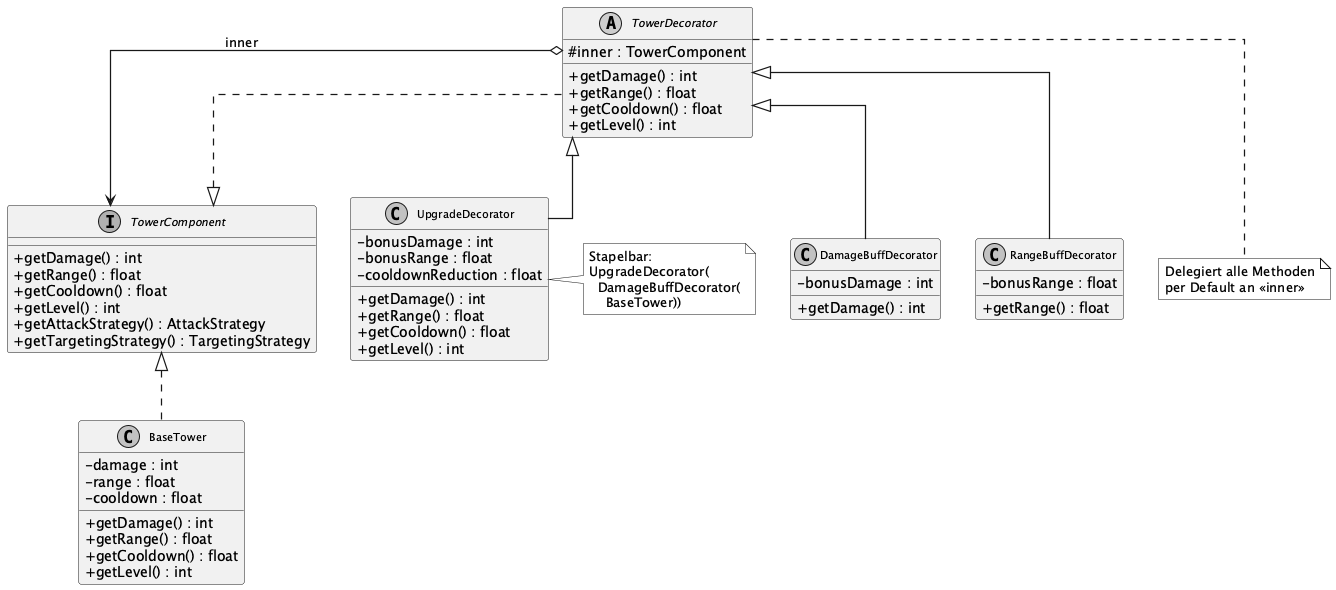
\includegraphics[width=\textwidth]{diagrams/decorator}
    \caption{Decorator-Pattern: \texttt{TowerComponent}-Hierarchie mit stapelbaren Dekoratoren}
    \label{fig:decorator}
\end{figure}

Dekoratoren lassen sich beliebig stapeln. Ein Aufruf von \texttt{getDamage()}
auf einem \texttt{UpgradeDecorator(DamageBuffDecorator(BaseTower))} traversiert
transparent die gesamte Kette und summiert alle Boni auf. Die restliche
Spiellogik, Strategy und GameManager, sieht stets nur ein
\texttt{TowerComponent} und muss nichts von der Decorator-Kette wissen.
Neue Bufftypen lassen sich vollständig ohne Änderung bestehender Klassen
ergänzen.

% =============================================================================
\subsection{Command - Kartensystem}
% =============================================================================

Das Command-Pattern kapselt jede Spielaktion als eigenständiges Objekt. Die
abstrakte Basisklasse \texttt{Card} definiert das Command-Interface mit der
Methode \texttt{execute(CardContext)}. Jede konkrete Kartenklasse ist ein
ConcreteCommand: Sie kennt ausschließlich ihren eigenen Parameter, etwa den
Schadenswert oder die Langsamdauer, und delegiert die Ausführung vollständig
an den Receiver.

Der \texttt{GameManager} übernimmt die Receiver-Rolle. Er stellt für jede
Spielaktion eine semantisch benannte Methode bereit:
\texttt{applyDamageBuff()}, \texttt{queueRangeBuff()} und
\texttt{slowAllEnemies()} kapseln die jeweilige Implementierungslogik, etwa
die Konstruktion von Decorator-Objekten oder die Iteration über die
Gegnerliste. Die Karten wissen \textit{was} ausgelöst werden soll, der
\texttt{GameManager} weiß \textit{wie} es intern umgesetzt wird.

\begin{lstlisting}[caption={Command-Pattern: DamageBuffCard delegiert an den Receiver},label=lst:command]
// ConcreteCommand kennt nur seinen Parameter
public void execute(CardContext context) {
    context.getManager().applyDamageBuff(bonusDamage);
}

// Receiver kennt die Implementierungsdetails
public void applyDamageBuff(int bonusDamage) {
    applyTowerModifier(tower -> new DamageBuffDecorator(tower, bonusDamage));
}
\end{lstlisting}

Der \texttt{GameScreen} agiert als Invoker: Er ruft \texttt{playCard(index)}
auf dem \texttt{GameManager} auf, ohne konkrete Kartentypen zu kennen.
Die acht Kartenklassen, \texttt{DamageBuffCard}, \texttt{RangeBuffCard},
\texttt{FreezeCard}, \texttt{EnergyCard}, \texttt{GoldCard}, \texttt{DrawCard},
\texttt{DiscountCard} und \texttt{BuildTowerCard}, sind alle nach demselben
Prinzip aufgebaut: ein schlankes Aktionsobjekt, ein Receiver-Aufruf.

Das Command-Pattern kooperiert eng mit dem Decorator-Pattern:
\texttt{applyDamageBuff()} und \texttt{queueRangeBuff()} sind die einzigen
Stellen im System, an denen Decorator-Objekte erzeugt werden. Die Karten
kennen \textit{dass} ein Buff stattfindet, nicht \textit{wie} er durch
gestapelte Wrapper realisiert wird. Eine \texttt{undo()}-Methode auf dem
Command-Interface ist nicht implementiert, da Decorator-Ketten nicht trivial
rückgängig gemacht werden können.

% =============================================================================
\subsection{Strategy - Zielwahl und Angriffsverhalten}
% =============================================================================

Turmtypen unterscheiden sich in zwei voneinander unabhängigen Dimensionen:
\textit{wen} sie angreifen (Zielwahl) und \textit{wie} sie angreifen
(Angriffstyp). Scout und Sniper verwenden Einzelschuss, Rapid verteilt
Flächenschaden. Scout priorisiert den Gegner mit dem größten Fortschritt auf dem
Pfad, Sniper den mit den meisten Lebenspunkten. Diese Dimensionen sind
orthogonal, jede Kombination ist denkbar und sinnvoll einsetzbar.

Würde man diese Unterschiede direkt in den Turmklassen codieren, etwa durch
eine \texttt{switch}-Anweisung über den Turmtyp, müsste bei jedem neuen Turmtyp
oder jeder neuen Angriffsvariante die Turmklasse geändert werden. Das verletzt
das Single-Responsibility Principle und führt zu wachsenden, schwer lesbaren
Klassen.

Das Strategy-Pattern trennt die beiden Dimensionen in zwei Interfaces:
\texttt{TargetingStrategy} kapselt die Zielwahl, \texttt{AttackStrategy} die
Angriffsausführung. Jeder Turm erhält bei seiner Erzeugung durch die
\texttt{StrategyCardFactory} eine konkrete Kombination beider Strategien und
delegiert beim Feuern vollständig an sie. Die vier möglichen Kombinationen
aus zwei Targeting- und zwei Angriffsstrategien entstehen ohne eine einzige
zusätzliche Klasse.

\begin{figure}[H]
    \centering
    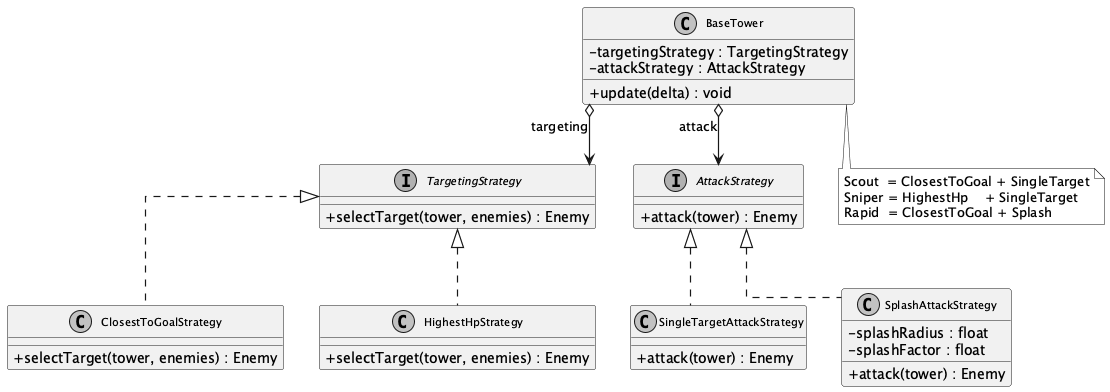
\includegraphics[width=\textwidth]{diagrams/strategy}
    \caption{Strategy-Pattern: zwei orthogonale Verhaltens-Dimensionen, zusammengeführt im \texttt{BaseTower}}
    \label{fig:strategy}
\end{figure}

Das Zusammenspiel mit dem Decorator-Pattern ist besonders subtil: Wenn die
\texttt{SplashAttackStrategy} \texttt{tower.getDamage()} aufruft, traversiert
dieser Aufruf transparent eine möglicherweise mehrschichtige Decorator-Kette.
Die Strategie erhält stets den kumulierten, gebufften Schadenswert, ohne davon
zu wissen. Die Entkopplung funktioniert vollständig über das gemeinsame Interface
\texttt{TowerComponent}.

% =============================================================================
\subsection{State - Spielphasenzyklus}
% =============================================================================

Der Spielablauf gliedert sich in einen geschlossenen Viererzyklus:
\textit{Draw} $\rightarrow$ \textit{Play} $\rightarrow$ \textit{Wave}
$\rightarrow$ \textit{Resolve} $\rightarrow$ \textit{Draw} $\rightarrow$ \ldots\
Jede Phase bringt eigene Regeln mit: In der Draw-Phase werden Karten gezogen und
Energie aufgefüllt, in der Play-Phase spielt der Spieler Karten aus und
positioniert Türme, in der Wave-Phase läuft die Gegnerwelle während Buff-Karten
weiterhin einsetzbar sind, und die Resolve-Phase leitet nach kurzem Delay den
nächsten Zug ein. Zwölf abgeschlossene Wellen führen zum Sieg, fehlende
Basislebenspunkte zur Niederlage.

Ohne das State-Pattern würde der \texttt{GameManager} ein wachsendes Geflecht
aus phasenabhängigen Bedingungen verwalten: Karten dürfen nur in bestimmten
Phasen ausgespielt werden, Gegner spawnen nur in der Wave-Phase, der nächste Zug
beginnt erst nach Ablauf eines Timers. All dieses Verhalten in einer einzigen
Klasse zu konzentrieren würde zu unübersichtlichen
\texttt{if~(currentPhase~==~...)}-Ketten führen, die mit jeder neuen Phase
schwerer wartbar werden.

Das State-Pattern kapselt das Verhalten jeder Phase vollständig in einer eigenen
Klasse, die das Interface \texttt{GamePhase} implementiert. Dieses schreibt drei
Methoden vor: \texttt{getName()} liefert den Phasennamen, \texttt{enter()} wird
einmalig beim Betreten der Phase aufgerufen und enthält Initialisierungslogik,
\texttt{update()} wird in jedem Frame aufgerufen und enthält das laufende
Verhalten. Der \texttt{GameManager} kennt keine Phasenlogik, er ruft lediglich
\texttt{phase.update()} auf und wechselt die Phase auf Anforderung.

\begin{lstlisting}[caption={Phasenwechsel im GameManager und Beispielphase},label=lst:state]
// GameManager delegiert vollstaendig an die aktive Phase:
public void switchPhase(GamePhase newPhase) {
    this.phase = newPhase;
    newPhase.enter(this);
    eventBus.publish(GameEvent.phaseChanged(newPhase.getName()));
}

// DrawPhase initialisiert den Zug und wechselt sofort weiter:
public void enter(GameManager manager) {
    manager.drawHand(3);
    manager.resetEnergy(3);
    manager.switchPhase(new PlayPhase());
}
\end{lstlisting}

\begin{figure}[H]
    \centering
    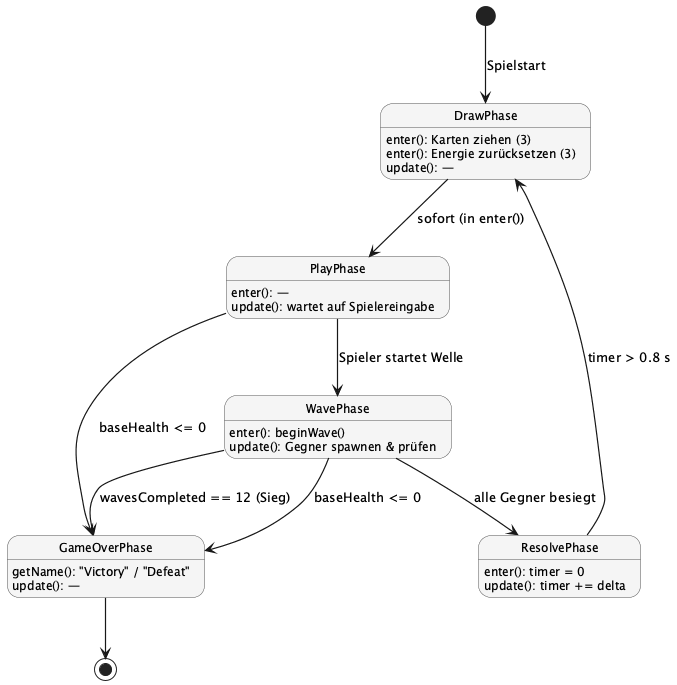
\includegraphics[width=0.82\textwidth]{diagrams/state}
    \caption{State-Pattern: Zustandsübergänge im Spielphasenzyklus}
    \label{fig:state}
\end{figure}

Die fünf Phasenklassen zeigen, wie sauber das Verhalten lokalisiert ist. Die
\texttt{DrawPhase} hat eine leere \texttt{update()}-Methode, weil sie ihre
gesamte Logik in \texttt{enter()} abarbeitet und sofort weiterleitet. Die
\texttt{PlayPhase} hat leere Implementierungen beider Methoden, weil sie
ausschließlich auf externe Nutzerinteraktion wartet, der Übergang in die
\texttt{WavePhase} wird vom \texttt{GameScreen} ausgelöst. Die
\texttt{ResolvePhase} verwaltet einen internen Timer und löst nach 0,8~Sekunden
selbstständig den nächsten Zug aus. Die \texttt{GameOverPhase} schließlich
bleibt in beiden Methoden leer: Das Spiel ist eingefroren, kein automatischer
Übergang findet statt. Dass jede Phase exakt die Methoden füllt, die sie
braucht, und alle anderen leer lässt, macht das phasenspezifische Verhalten
auf einen Blick sichtbar.

Das State-Pattern kooperiert unmittelbar mit dem Observer-Pattern: Jeder Aufruf
von \texttt{switchPhase()} publiziert automatisch ein \texttt{PhaseChanged}-Event
über den \texttt{GameEventBus}, ohne dass die aufrufende Phase davon wissen muss.

% =============================================================================
\subsection{Observer - GameEventBus}
% =============================================================================

Im Spielverlauf entstehen kontinuierlich bedeutsame Ereignisse: Ein Turm wird
gebaut, ein Gegner besiegt, eine Phase wechselt, die Basis erleidet Schaden.
Systeme wie ein Logger, ein Sound-Modul oder ein Statistik-Tracker sollen auf
diese Ereignisse reagieren, ohne dass der \texttt{GameManager} direkte
Abhängigkeiten zu ihnen aufbaut. Würde der Manager Logger oder UI direkt
referenzieren, entstünde enge Kopplung: Jede neue reaktive Komponente würde
Manager-Code erzwingen und die Klasse weiter aufblähen.

Das Observer-Pattern kehrt diese Abhängigkeit um. Der \texttt{GameEventBus}
verwaltet eine Liste von \texttt{GameEventListener}-Implementierungen und
benachrichtigt sie synchron bei jedem publizierten Ereignis. Die Abhängigkeit
zeigt nun in die entgegengesetzte Richtung: Nicht der Manager kennt den Logger,
sondern der Logger registriert sich selbst am Manager, zur Initialisierungszeit,
im privaten Singleton-Konstruktor.

Statt einfacher String-Konstanten verwendet das System typisierte Factory-Methoden
auf der \texttt{GameEvent}-Klasse: \texttt{GameEvent.towerBuilt(x,~y)},
\texttt{GameEvent.phaseChanged(name)} oder \texttt{GameEvent.baseDamaged(hp)}.
Diese Methoden konstruieren Events auf lesbare Weise und verhindern die Streuung
von Magic-Strings über die Codebasis. Gleichzeitig bleibt \texttt{GameEvent}
ein einfaches Wertobjekt ohne Vererbungshierarchie, der Ereignisname trägt
alle nötigen Informationen.

Aktuell ist der \texttt{GameEventLogger} der einzige Subscriber; er schreibt
jedes Ereignis auf die Konsole und macht den Spielverlauf nachvollziehbar. Die
Architektur ist dabei bereits für Erweiterungen offen: Ein Achievement-System,
ein Sound-Manager oder ein Replay-Recorder könnten sich mit einem einzigen
\texttt{eventBus.subscribe()}-Aufruf registrieren, ohne eine Zeile im
\texttt{GameManager} oder in bestehenden Listenern zu ändern. Das
Observer-Pattern liefert damit eine Infrastruktur, deren Erweiterbarkeit weit
über den aktuellen Nutzungsumfang hinausgeht.

\newpage
% =============================================================================
% Kapitel 4 -- Implementierung: Relevante Funktionen
% =============================================================================
\section{Implementierung}

Dieses Kapitel beschreibt stichpunktartig die zentralen Funktionen und Subsysteme
von CardSiege. Im Vordergrund steht, was die einzelnen Komponenten leisten, die
zugrundeliegenden Architektur- und Pattern-Entscheidungen wurden in Kapitel~3
erläutert.

% -----------------------------------------------------------------------------
\subsection{Spielzustand und Frame-Loop}
% -----------------------------------------------------------------------------

Der \texttt{GameManager} verwaltet als zentrales Singleton den gesamten
Spielzustand und koordiniert alle Subsysteme. Die Methode \texttt{init(board, cardFactory)}
setzt alle Zustandsvariablen zurück, initialisiert Deck und Hand und startet mit
Startressourcen (3 Energie, 5 Gold, 10 Basislebenspunkte) in der
\texttt{DrawPhase}. Die Frame-Methode \texttt{update(delta)} ruft in fest
definierter Reihenfolge auf: Phasen-Update, Gegnerbewegung,
Reichweitenüberwachung, Turm-Update, Kampfauflösung, Entitätenbereinigung und
Projektilupdates.

Über \texttt{playCard(index)} wird die gewählte Karte aus der Hand entfernt,
Phase und Energieverfügbarkeit geprüft, der Energiebetrag abgezogen und
\texttt{card.execute()} aufgerufen. \texttt{BuildTowerCard}s sind während der
\texttt{WavePhase} gesperrt. Die Methoden \texttt{canPlayCard()} und
\texttt{getEffective\-Energy\-Cost()} kapseln alle Voraussetzungsprüfungen
(Phase, Energie, Gold, vorhandene Türme für Buff-Karten) sowie die Berechnung
aktiver Kartenrabatte.

% -----------------------------------------------------------------------------
\subsection{Turmsystem}
% -----------------------------------------------------------------------------

Über \texttt{queue\-Tower\-Placement(pending)} wird ein \texttt{PendingTower} gespeichert,
sobald ausreichend Gold vorhanden ist; der \texttt{GameScreen} rendert daraufhin
den Platzierungsmarker mit Reichweitenkreis. Beim Klick prüft \texttt{tryPlace\-Pending\-Tower(x, y)}
Baubarkeit des Feldes und ob es bereits belegt ist; bei Erfolg wird
\texttt{PendingTower.build()} aufgerufen, der Turm zur Liste hinzugefügt und Gold
abgezogen.

Beim Upgrade umhüllt \texttt{upgradeTower(tower)} den Turm mit einem
\texttt{UpgradeDecorator} (+1 Schaden, +15 Reichweite, reduzierter Cooldown); die
Kosten steigen pro Level (\texttt{2 + tower.getLevel()} Gold). Globale Buffs wie
\texttt{applyDamageBuff()} ersetzen jeden Turm in der Liste durch einen
entsprechenden Decorator-Wrapper. Für gezielte Buffs auf einzelne Türme speichert
\texttt{queueRangeBuff()} einen Factory-Auftrag, den
\texttt{tryApply\-Pending\-Tower\-Modifier()} beim nächsten vom Spieler ausgewählten
Turm anwendet.

Jeden Frame berechnet \texttt{update\-Range\-Observers()} per Quadratdistanzvergleich,
welche Gegner in Reichweite sind, und benachrichtigt den Turm über
Eintritte und Austritte. In \texttt{resolveCombat(delta)} wird über alle Türme
iteriert:
Bei \texttt{canFire()} wird \texttt{attack\-Strategy.attack()} aufgerufen, der
Cooldown zurückgesetzt und ein visuelles Projektil erzeugt.

% -----------------------------------------------------------------------------
\subsection{Gegnersystem und Kampf}
% -----------------------------------------------------------------------------

In \texttt{Enemy.update(delta)} bewegt sich der Gegner entlang der vorberechneten
Wegpunkt-Liste. Der \texttt{pathIndex} steigt, sobald ein Waypoint erreicht ist;
ein aktiver Slow-Effekt (\texttt{FreezeCard}) skaliert die Geschwindigkeit via
\texttt{slowFactor} für eine begrenzte Dauer. Per Quadratdistanzvergleich prüft \texttt{isInRange(tower)},
ob ein Gegner in Reichweite liegt; der Turmursprung liegt dabei in der
Kachelmitte.

Der \texttt{WaveSpawner} konfiguriert pro Welle drei
\texttt{EnemyPrototype}-Objekte mit skalierten Werten und spawnt Gegner in festen
Zeitintervallen. Sind alle Gegner gespawnt und die Gegnerliste leer, löst
\texttt{endWaveIfComplete()} den Übergang in die \texttt{ResolvePhase} oder
nach zwölf Wellen in die \texttt{GameOverPhase(true)} aus.

Nach jedem Frame bereinigt \texttt{cleanupEntities()} tote Gegner (+1 Gold,
\texttt{EnemyDefeated}-Event) und Gegner, die das Ziel erreicht haben
($-1$ Basislebenspunkt, \texttt{baseDamaged}-Event). Vor dem Entfernen werden
alle Turm-Observer über \texttt{remove\-Enemy\-From\-Observers()} benachrichtigt. Fällt
\texttt{baseHealth} auf null, wechselt das Spiel in \texttt{GameOverPhase(false)}.

% -----------------------------------------------------------------------------
\subsection{Kartensystem}
% -----------------------------------------------------------------------------

Beim Kartenziehen liefert \texttt{Deck.draw()} die oberste Karte; ist der Stapel leer, füllt
\texttt{refill()} ihn über Factory und Prototype-Klonen neu auf und mischt ihn
anschließend. \texttt{Hand} verwaltet die Handkarten als Liste;
\texttt{addToFront()} wird beim Zurücklegen einer abgelehnten Karte genutzt.

Zu Spielbeginn garantiert \texttt{ensure\-First\-Hand\-Has\-Tower()}, dass die erste Hand
mindestens eine \texttt{BuildTowerCard} enthält: Ist keine vorhanden,
wird die erste Handkarte an den Stapelboden gelegt und der Stapel nach einer
Turmkarte durchsucht. Über \texttt{addNext\-Card\-Discount(amount)} werden
Rabatt-Mechaniken der \texttt{DiscountCard} realisiert; der Rabatt wird nach dem nächsten
Kartenspielen auf null zurückgesetzt.

% -----------------------------------------------------------------------------
\subsection{Ereignissystem}
% -----------------------------------------------------------------------------

Der \texttt{GameEventBus} verwaltet eine Liste von
\texttt{Game\-Event\-Listener}-Implementierungen und benachrichtigt alle Subscriber
synchron per \texttt{publish()}. \texttt{GameEvent} ist ein einfaches Wertobjekt
mit typisierten Factory-Methoden (\texttt{towerBuilt(x,y)},
\texttt{phaseChanged(name)}, \texttt{baseDamaged(hp)}, \texttt{EnemyDefeated},
\texttt{cardPlayed(name)}), die Magic-Strings im gesamten System vermeiden. Der
\texttt{GameEventLogger} als einziger aktiver Subscriber schreibt jedes Ereignis
auf die Konsole; weitere Subscriber (Sound, Achievements) könnten ohne Änderung
am Bus per \texttt{subscribe()} ergänzt werden.

% -----------------------------------------------------------------------------
\subsection{Spielfeld und Pfadgenerierung}
% -----------------------------------------------------------------------------

\texttt{Tile} repräsentiert eine einzelne Kachel mit Gitterkoordinaten und
einem booleschen \texttt{path}-Flag. \texttt{Board} hält die Kachelliste,
die vorberechnete Pfad-Vektorliste und stellt \texttt{isBuildable(gridX,~gridY)}
für Bauprüfungen bereit.

Der Pfad wird einmalig in \texttt{Board.createDefault()} erzeugt: Zwölf
relativ zur Spielfeldgröße skalierte Kontrollpunkte werden durch
ausschließlich horizontale und vertikale Segmente verbunden. Die resultierenden
Gitterkoordinaten landen als \texttt{GridPoint}-Records in einem
\texttt{LinkedHashSet}, das Duplikate entfernt und die Reihenfolge erhält. Jede Koordinate wird als
\texttt{Tile(path=true)} markiert und als Weltkoordinate in die Pfad-Liste
übernommen, entlang derer Gegner sich bewegen.

% -----------------------------------------------------------------------------
\subsection{Projektile}
% -----------------------------------------------------------------------------

Als reines Darstellungsobjekt speichert \texttt{Projectile} Start- und Zielposition
sowie eine \texttt{ttl}-Zeit von 0,15~Sekunden; die Spiellogik bleibt davon
unberührt. Für weiches Ausblenden liefert \texttt{getAlpha()} einen linear
abfallenden Transparenzwert; \texttt{isExpired()}
signalisiert dem \texttt{GameManager} das Entfernen aus der Liste. Schaden und
Trefferauswertung sind bereits in \texttt{resolveCombat()} abgeschlossen,
bevor das Projektil erzeugt wird.

% -----------------------------------------------------------------------------
\subsection{Benutzeroberfläche und Eingabe}
% -----------------------------------------------------------------------------

Der \texttt{GameScreen} bildet die einzige Verbindung zwischen Spiellogik und
Darstellung. Pro Frame delegiert \texttt{render()} zunächst \texttt{update(delta)} an
den \texttt{GameManager} und zeichnet danach Hintergrund, Spielfeld, Entitäten,
Platzierungsvorschau und HUD. Türme erscheinen als farbige Rechtecke, Gegner
als Kreise mit HP-Balken, Projektile als gelbe Linien mit \texttt{alpha}-Ausblenden.

Aktiv ist \texttt{drawPlacementPreview()}, solange ein \texttt{PendingTower}
im Manager registriert ist: Das überfahrene Feld wird grün (baubar) oder rot
(gesperrt) eingefärbt, ein Reichweitenkreis zeigt die Abdeckung -- ohne dass
ein echter Turm existiert. Das HUD zeigt Ressourcen und Handkarten; spielbare
Karten werden grün, nicht spielbare rot hinterlegt. Über \texttt{collectBuffs()}
wird die Decorator-Kette eines selektierten Turms traversiert und alle
aktiven Boni für das Tooltip summiert.

Die innere Klasse \texttt{GameInputProcessor} übernimmt die Eingabe:
\texttt{[1--8]} spielen Karten, \texttt{SPACE} startet die Welle, \texttt{U}
upgraded den selektierten Turm, \texttt{R} startet neu und \texttt{ESC} kehrt
zum Menü zurück. Mausklicks werden per \texttt{camera.unproject()} in
Gitterkoordinaten konvertiert und lösen je nach Zustand
\texttt{tryPlace\-PendingTower()} oder \texttt{tryApply\-Pending\-Tower\-Modifier()} aus.

\newpage
% =============================================================================
% Kapitel 5 -- Zusammenfassung und Fazit
% =============================================================================
\section{Zusammenfassung und Fazit}

\subsection{Ergebnisse}

CardSiege ist ein vollständiges, spielbares Kartenspiel, das alle funktionalen
Anforderungen erfüllt und neun GoF-Design-Patterns sinnvoll integriert. Die vier
Erzeugungsmuster -- Singleton, Factory Method, Prototype und Builder -- strukturieren
gemeinsam die gesamte Objekterzeugung des Spiels: Der Singleton sichert den
konsistenten Spielzustand, die Factory entkoppelt das Deck von konkreten
Kartentypen, das Prototype-Pattern ermöglicht effizientes Klonen konfigurierter
Objekte, und der Builder trennt Turmkonfiguration von Platzierung. Das
Decorator-Pattern als einziges Strukturmuster löst das zentrale Erweiterungsproblem
im Turmsystem. Die vier Verhaltensmuster -- Command, Strategy, State und Observer --
modellieren das laufende Spielgeschehen so, dass Erweiterungen ohne Modifikation
bestehender Klassen möglich sind.

\subsection{Erkenntnisse und Grenzen}

Die Arbeit hat gezeigt, dass Design Patterns erst im Kontext eines realen Problems
ihren vollen Wert entfalten. Das Decorator-Pattern wirkt in der Theorie
überengineert -- erst das Skizzieren der alternativen Vererbungshierarchie macht
den konkreten Mehrwert sichtbar. Das Strategy-Pattern reduziert eine potentiell
komplexe Fallunterscheidung im Turmangriff auf zwei austauschbare Algorithmen,
die sich ohne Seiteneffekte kombinieren lassen.

Besonders aufschlussreich war das natürliche Zusammenspiel der Patterns: Factory
und Prototype kooperieren im Deck, State und Observer im Phasenzyklus, Command
und Decorator im Buff-Kartensystem. Die Patterns verstärken sich gegenseitig --
keine Lösung ist in sich geschlossen, alle greifen ineinander.

Grenzen wurden ebenfalls sichtbar. Das Singleton erschwert Unit-Tests durch
persistierenden Zustand. Der \texttt{GameManager} trägt trotz aller Delegation
noch sehr viele Verantwortlichkeiten; in einem größeren Projekt würde man ihn in
separate \texttt{CombatManager}- und \texttt{ResourceManager}-Klassen aufteilen.

\subsection{Ausblick}

Das System bietet konkrete Ansatzpunkte für Erweiterungen, die unmittelbar auf
der bestehenden Architektur aufbauen. Konfigurierbare Decks und ein
Progressionssystem, bei dem nach und nach neue Karten freigeschaltet werden,
ließen sich vollständig über das Factory-Pattern realisieren: Jede
Fortschrittsstufe entspräche einer neuen \texttt{CardFactory}-Implementierung,
ohne eine Zeile in \texttt{Deck} oder den bestehenden Karten zu ändern. Neue
Gegner- und Turmtypen sind durch \texttt{EnemyPrototype} beziehungsweise
\texttt{StrategyCardFactory} bereits architektonisch vorbereitet -- das
Hinzufügen eines weiteren Eintrags genügt.

Das Command-Pattern legt die Grundlage für eine Undo-Funktion: Eine
\texttt{undo()}-Methode auf \texttt{Card} würde Kartenaktionen rückgängig
machbar machen, was gerade für ein Progressionssystem mit begrenzten Ressourcen
spielerisch wertvoll wäre. Das Memento-Pattern böte eine elegante Basis für
Spielstand-Speicherung. Ein Endless-Mode schließlich ließe sich mit minimalen
Eingriffen umsetzen: \texttt{WaveSpawner} und \texttt{GameOverPhase} müssten
lediglich die feste Wellenobergrenze durch eine unbegrenzte Skalierungslogik
ersetzen, alle anderen Systeme blieben unverändert.

\newpage
\section*{Erklärung}
\markboth{Erklärung}{Erklärung}

Ich erkläre hiermit, dass ich die vorliegende Arbeit selbstständig verfasst und dabei keine anderen als die angegebenen Hilfsmittel benutzt habe. Sämtliche Stellen der Arbeit, die im Wortlaut oder dem Sinn nach Werken anderer Autoren entnommen sind, habe ich als solche kenntlich gemacht. Die Arbeit wurde bisher  noch nicht einer anderen Prüfungsbehörde vorgelegt und auch noch nicht veröffentlicht.

\bigskip
\noindent
\datum

\vspace{25mm}

\noindent


\vspace{25mm}

Sven Sinowczik

Matrikelnummer: 30422906

\end{document}
